% Auto-generated by intrusion_detection. Do not edit manually.
\newcommand{\ResultAdfaLdPagerankAccuracy}{0.8128}
\newcommand{\ResultAdfaLdPagerankFOne}{0.4652}
\newcommand{\ResultAdfaLdPagerankPrecision}{0.3619}
\newcommand{\ResultAdfaLdPagerankRecall}{0.6510}
\newcommand{\ResultAdfaLdPagerankRocAuc}{0.8092}
\newcommand{\ResultAdfaLdPagerankSupport}{1191}
\newcommand{\ResultAdfaLdWgcnPlusAccuracy}{0.9244}
\newcommand{\ResultAdfaLdWgcnPlusFOne}{0.7289}
\newcommand{\ResultAdfaLdWgcnPlusPrecision}{0.6612}
\newcommand{\ResultAdfaLdWgcnPlusRecall}{0.8121}
\newcommand{\ResultAdfaLdWgcnPlusRocAuc}{0.9636}
\newcommand{\ResultAdfaLdWgcnPlusSupport}{1191}
\newcommand{\ResultAdfaLdGcnAccuracy}{0.9362}
\newcommand{\ResultAdfaLdGcnFOne}{0.7164}
\newcommand{\ResultAdfaLdGcnPrecision}{0.8067}
\newcommand{\ResultAdfaLdGcnRecall}{0.6443}
\newcommand{\ResultAdfaLdGcnRocAuc}{0.9567}
\newcommand{\ResultAdfaLdGcnSupport}{1191}
\newcommand{\ResultAdfaLdGraphsageAccuracy}{0.9337}
\newcommand{\ResultAdfaLdGraphsageFOne}{0.7208}
\newcommand{\ResultAdfaLdGraphsagePrecision}{0.7612}
\newcommand{\ResultAdfaLdGraphsageRecall}{0.6846}
\newcommand{\ResultAdfaLdGraphsageRocAuc}{0.9617}
\newcommand{\ResultAdfaLdGraphsageSupport}{1191}
\newcommand{\ResultAdfaLdGatAccuracy}{0.9488}
\newcommand{\ResultAdfaLdGatFOne}{0.7987}
\newcommand{\ResultAdfaLdGatPrecision}{0.7857}
\newcommand{\ResultAdfaLdGatRecall}{0.8121}
\newcommand{\ResultAdfaLdGatRocAuc}{0.9790}
\newcommand{\ResultAdfaLdGatSupport}{1191}
\newcommand{\ResultLidBruteforcePagerankAccuracy}{0.9890}
\newcommand{\ResultLidBruteforcePagerankFOne}{0.9630}
\newcommand{\ResultLidBruteforcePagerankPrecision}{1.0000}
\newcommand{\ResultLidBruteforcePagerankRecall}{0.9286}
\newcommand{\ResultLidBruteforcePagerankRocAuc}{1.0000}
\newcommand{\ResultLidBruteforcePagerankSupport}{182}
\newcommand{\ResultLidBruteforceWgcnPlusAccuracy}{0.9560}
\newcommand{\ResultLidBruteforceWgcnPlusFOne}{0.8462}
\newcommand{\ResultLidBruteforceWgcnPlusPrecision}{0.9167}
\newcommand{\ResultLidBruteforceWgcnPlusRecall}{0.7857}
\newcommand{\ResultLidBruteforceWgcnPlusRocAuc}{0.9666}
\newcommand{\ResultLidBruteforceWgcnPlusSupport}{182}
\newcommand{\ResultLidCvePagerankAccuracy}{0.8864}
\newcommand{\ResultLidCvePagerankFOne}{0.3750}
\newcommand{\ResultLidCvePagerankPrecision}{0.7500}
\newcommand{\ResultLidCvePagerankRecall}{0.2500}
\newcommand{\ResultLidCvePagerankRocAuc}{0.7818}
\newcommand{\ResultLidCvePagerankSupport}{176}
\newcommand{\ResultLidCveWgcnPlusAccuracy}{0.8636}
\newcommand{\ResultLidCveWgcnPlusFOne}{0.0000}
\newcommand{\ResultLidCveWgcnPlusPrecision}{0.0000}
\newcommand{\ResultLidCveWgcnPlusRecall}{0.0000}
\newcommand{\ResultLidCveWgcnPlusRocAuc}{0.9380}
\newcommand{\ResultLidCveWgcnPlusSupport}{176}

\subsection{Automated Results}
\begin{table}[t]
\centering
\resizebox{\linewidth}{!}{%
\begin{tabular}{lllrrrrr}
\hline
Dataset & Scenario & Model & Acc. & F1 & Prec. & Rec. & ROC-AUC \\
\hline
adfa\_ld & all & pagerank & 0.8128 & 0.4652 & 0.3619 & 0.6510 & 0.8092 \\
adfa\_ld & all & gnn:wgcn\_plus & 0.9244 & 0.7289 & 0.6612 & 0.8121 & 0.9636 \\
adfa\_ld & all & gnn:gcn & 0.9362 & 0.7164 & 0.8067 & 0.6443 & 0.9567 \\
adfa\_ld & all & gnn:graphsage & 0.9337 & 0.7208 & 0.7612 & 0.6846 & 0.9617 \\
adfa\_ld & all & gnn:gat & 0.9488 & 0.7987 & 0.7857 & 0.8121 & 0.9790 \\
lid\_ds & Bruteforce\_CWE-307 & pagerank & 0.9890 & 0.9630 & 1.0000 & 0.9286 & 1.0000 \\
lid\_ds & Bruteforce\_CWE-307 & gnn:wgcn\_plus & 0.9560 & 0.8462 & 0.9167 & 0.7857 & 0.9666 \\
lid\_ds & CVE-2014-0160 & pagerank & 0.8864 & 0.3750 & 0.7500 & 0.2500 & 0.7818 \\
lid\_ds & CVE-2014-0160 & gnn:wgcn\_plus & 0.8636 & 0.0000 & 0.0000 & 0.0000 & 0.9380 \\
\hline
\end{tabular}
}
\caption{Test-set metrics exported automatically from the training pipeline.}
\label{tab:automated-results}
\end{table}

\subsection{Diagnostics: adfa\_ld\_pagerank}
\begin{figure}[t]
\centering
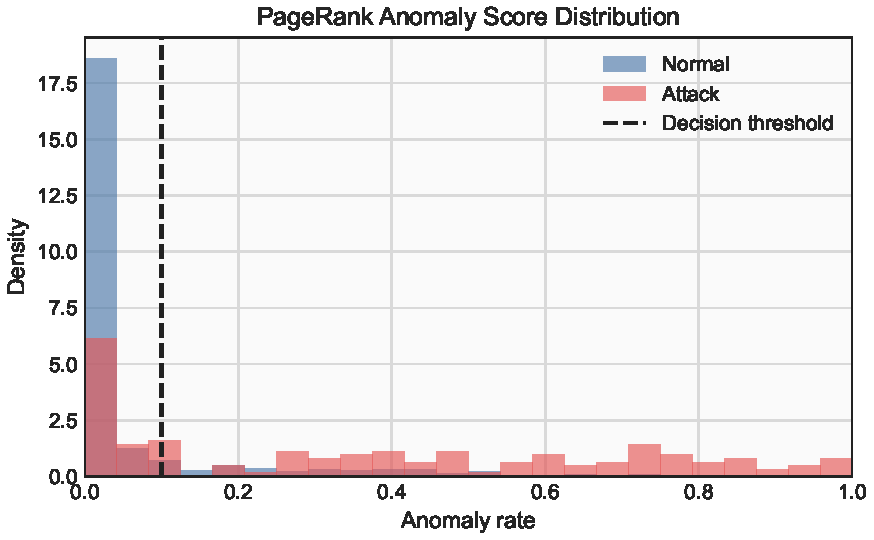
\includegraphics[width=0.7\linewidth]{figures/adfa_ld_pagerank_scores.pdf}
\caption{Diagnostic plot for \texttt{adfa\_ld\_pagerank}: distribution of test anomaly scores with the decision threshold.}
\end{figure}
\subsection{Diagnostics: adfa\_ld\_gat}
\begin{figure}[t]
\centering
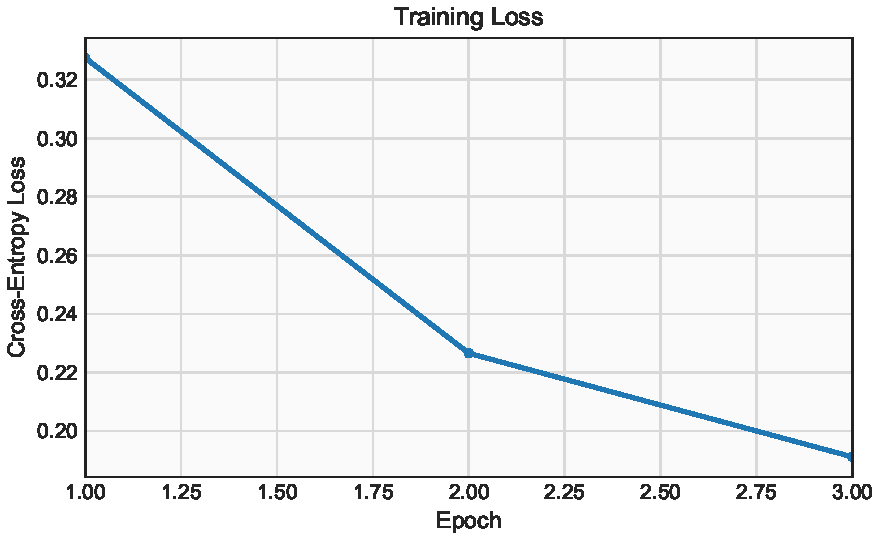
\includegraphics[width=0.48\linewidth]{figures/adfa_ld_gat_loss.pdf}
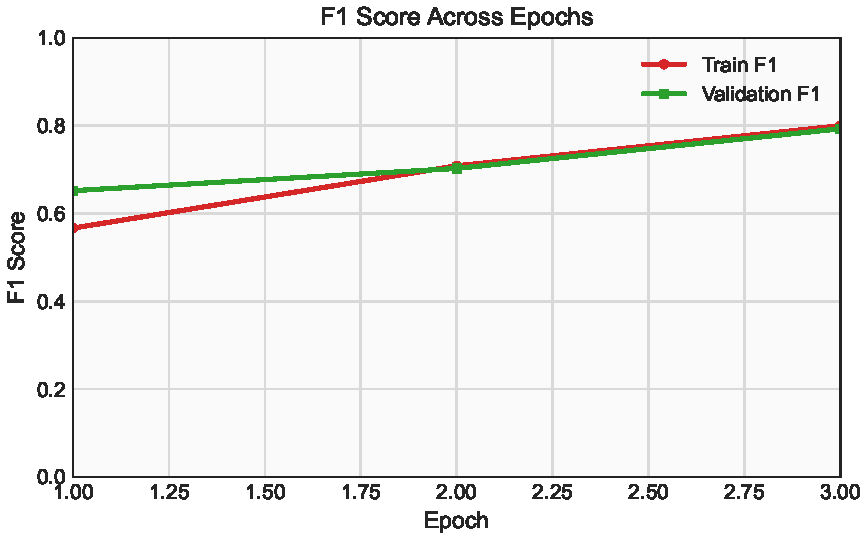
\includegraphics[width=0.48\linewidth]{figures/adfa_ld_gat_f1.pdf}
\caption{Training diagnostics for \texttt{adfa\_ld\_gat}: cross-entropy loss and F1 score as a function of epoch.}
\end{figure}
